\section{Functional Improvements}
	\subsection{Swap Time}
		\subsubsection{Experiment Description}
		\subsubsection{Results}
		\subsubsection{Analysis}
	\subsection{Compatibility}
\section{Signal Quality Verifications}

The second main category of system verification measurements are related to maintaining the same signal integrity as if the guitar were connected directly to the amplifier using an instrument cable.  This allows users to make objective and unbiased comparisons between the products being tested.

	\subsection{Signal-to-Noise Ratio}
		\subsubsection{Measurement Description}
		For this test, an Audio Precision System One (AP) measurement device was used to measure the noise floor of the device under test.  The AP and associated software was used to send programmable test signals through the device and measure the resulting response.  To measure the noise floor, the AP was programmed to output a sinusoid test signal and the amplitude was swept from $+10 dBu$ down to $-100 dBu$.  This corresponds to a sweep from a $6.9Vpp$ signal down to $22\mu Vpp$.

		The plots in Figure \ref{fig:NF_AP} show the amplitude of the measured signal (in $dBu$) plotted against this swept test signal.  When the test signal is above the noise floor, its amplitude dominates the output and the plot shows a straight line with a unit slope.  However, when the test signal's amplitude goes below the noise floor, this dominates, and the slope goes to zero, indicating the level of the noise floor at the measured level of this flat part of the plot.

		The first measurement made was a characterization of the AP itself, with its output and input connected with a two foot coaxial cable.  Measuring the AP's own noise floor shows the limits of observation with this device.

		The important data measurements were then conducted.  Two setups were used, as the signal path which passed only through relays was expected to have a different noise characteristic than the signal path which include the buffers and summing amplifier.

		\subsubsection{Results}

		\begin{figure}[!htbp]
			\centering
			\begin{subfigure}{0.66\textwidth}
				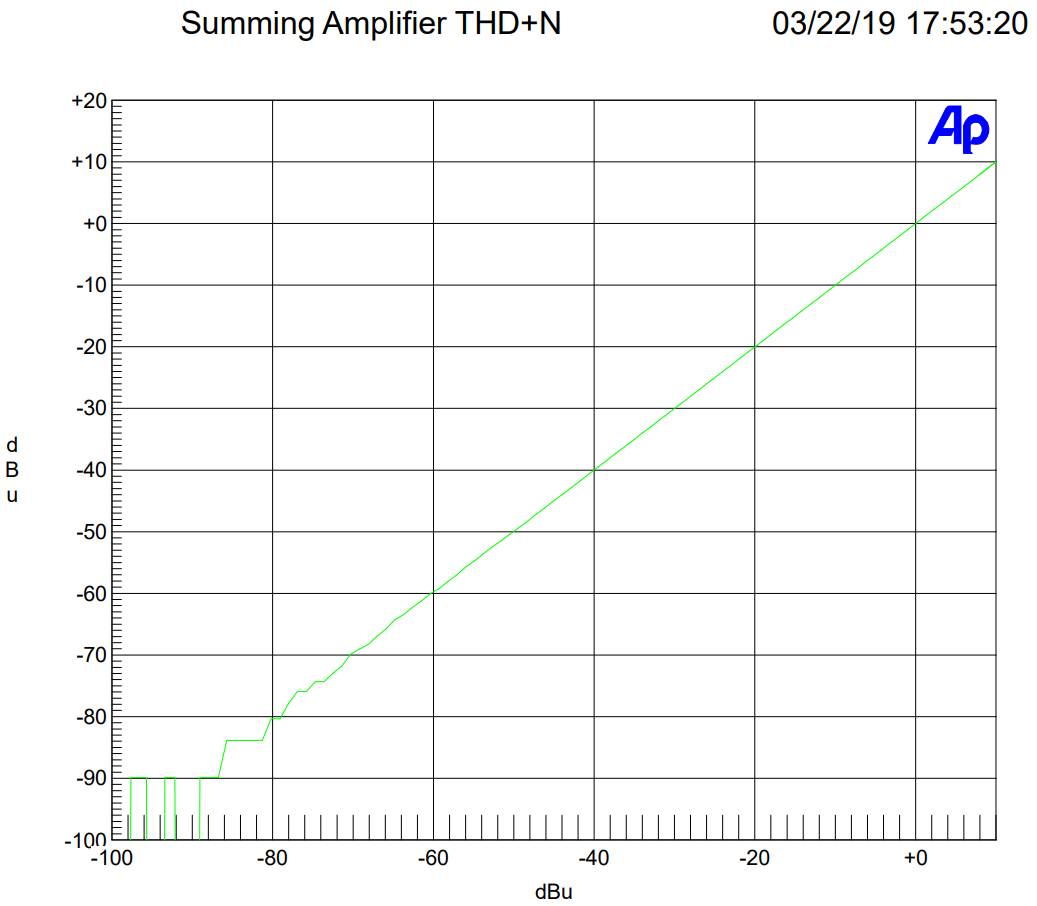
\includegraphics[width = \textwidth]{FinalImages/NF_direct.png}
				\caption{\emph{Direct} routing noise floor measurement output.}
				\label{fig:NF_AP_direct}
			\end{subfigure}
			\vspace{0.5in}
			\begin{subfigure}{0.66\textwidth}
				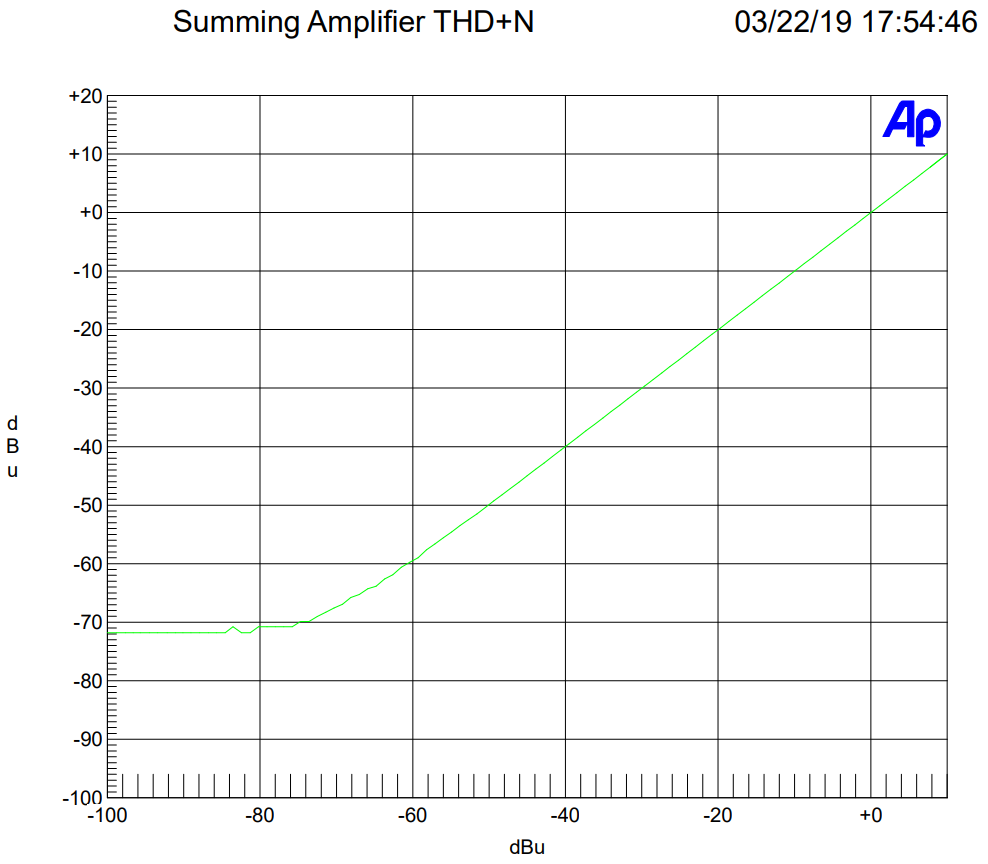
\includegraphics[width = \textwidth]{FinalImages/NF_sum.png}
				\caption{\emph{Summed} routing noise floor measurement output.}
				\label{fig:NF_AP_sum}
			\end{subfigure}
			\caption{Example AP noise floor measurement plots.  The x-axis shows the AP's test sinusoid output amplitude in $dBu$, and the y-axis shows the measured amplitude from the device under test.}
			\label{fig:NF_AP}
		\end{figure}

		During the first measurement, the external switching power supply which had been used was determined to be much more noisy than expected.  During measurements for the prototype in the fall semester, it did exhibit some noise issues, but they were only marginally detrimental to the noise performance.  However, during this test the power supply was demonstrating approximately a $77mV$ noise signal with a strong component near $330Hz$ (equivalent to $-29 dBu$, which resulted in far worse measured noise floor than expected.  The $330Hz$ location of the noise is not something that could be ignored because it is right in the fundamental frequency range of the guitar.  With this in mind, this power supply was replaced with a bench top power supply that did not exhibit any issues.  This lab power supply was used during the rest of the measurements to isolate noise from the device itself.  This is not an unreasonable substitution, as an alternative power supply with a better specification could be easily switched out in the future to solve this issue.

		Both the noise floor measurement from the \emph{direct} signal path which only includes mechanical relays and the measurement from the \emph{summed} signal pat is shown in Figure \ref{fig:SNRbar}.  The bars are referenced to the AP's own noise floor which sets the limit of this measurement.  Lower values indicate better noise performance.  As can be seen, the \emph{direct} signal path performs very well, while the \emph{summed} signal path has a higher noise floor.

		Figure \ref{fig:NF_AP} shows two of the plots generated by the AP software.  Note the strange oscillations in Figure \ref{fig:NF_AP_direct} below $-96dBu$ which suggest that the device's noise floor may be reaching the limits of the measurement system (the plots generated during the characterization of the AP itself showed similar behavior).  On the other hand, Figure \ref{fig:NF_AP_sum} shows more normal behavior of the noise floor overwhelming the test signal.

		\insertimage{0.8}{FinalImages/SNR_bargraph.png}{Results of the noise floor measurements.  The AP's own noise floor was measured to be $-107dBu$.  This was used as a reference value for the other measurements, so effectively the bars show the increase in noise floor over the minimum possible value to be measured; lower values indicate better noise performance.  The \emph{direct} signal path's noise floor was less than $10dBu$ off of the best measurable value, while the summing amplifier performed significantly worse at just $-72.2dBu$.  For all of these measurements, $N=20$ samples were taken.}{fig:SNRbar}


		\subsubsection{Analysis}

		Of course, the noise floor is only one part of the signal to noise ratio; also required is the maximum signal amplitude.  Although in theory the electro mechanical relays can conduct hundreds of volts, this would skew the results of this measurement as guitar pedals would not be expected to output that type of level.  Instead, a reasonable estimation of the maximum signal level would be an $18Vpp$ signal, which would be the largest expected signal from the guitar pedals being tested, as $18V$ is the maximum output of the adjustable regulators supply power to the pedals.  Although some pedals may have internal circuitry to boost their on-board supply voltages above this level, these are few and far between.

		To compute the signal to noise ratio from the measured noise floor and the approximate maximum signal level,

		\begin{align*}
			SNR &= \frac{A_{max}}{A_{noise}} \\
			&= \log(A_{max}) - log(A_{noise})
		\end{align*}

		subtract the noise floor in $dBu$ from the maximum signal level amplitude in $dBu$.  With the two noise floor values recorded in Figure \ref{fig:SNRbar}, the actual signal to noise ratio and can calculated:

		\begin{align*}
			{SNR}_{direct} &= 18.3 - (-96.4) = 114.7 dBu \\
			{SNR}_{summed} &= 18.3 - (-72.2) = 90.5 dBu
		\end{align*}

		Both of these values exceed the design requirement of $90 dBu$, though the \emph{summed} path does not exceed it by much.  These high signal to noise ratios, particular that of the direct, relay-only signal allows users to make informed decisions about the products they audition as they can be sure that this system adds negligible noise.


	\subsection{Frequency Response}
		\subsubsection{Measurement Description}
		The AP system was also used to conduct this test.  Again, the output of the AP was connected to the input of the device under test, and the output of the device under test was connected to the input of the AP.  Here, the AP was programmed to output a sine wave sweep from $50kHz$ down to $10Hz$ at a $0dBu$ amplitude, at 51 discrete frequencies. The AP measured the amplitude of the resulting device output and plotted this against frequency.

		\subsubsection{Results}

		Again, the frequency response was measured for both the \emph{direct} and \emph{summed} signal paths.  Figure \ref{fig:FR_AP} shows the results of the frequency response measurement for both signal paths.  The \emph{direct} signal path measurement in \ref{fig:FR_AP_direct} is very flat down to the minimum frequency.  In fact, the relays should work down to DC.  There is a slight roll off in the upper frequencies mainly above $20kHz$ which could be due to loading from the biasing components used for the summing amplifier and associated buffers.  On the other hand, the \emph{summed} signal path does have a noticeable roll-off in the low frequencies, which appears to start around $100Hz$.  This is a result of the decoupling capacitors used to bias the summing amplifier and buffers to the $A_{Vdd}/2$ virtual ground.

		\begin{figure}[!htbp]
			\centering
			\begin{subfigure}{0.6\textwidth}
				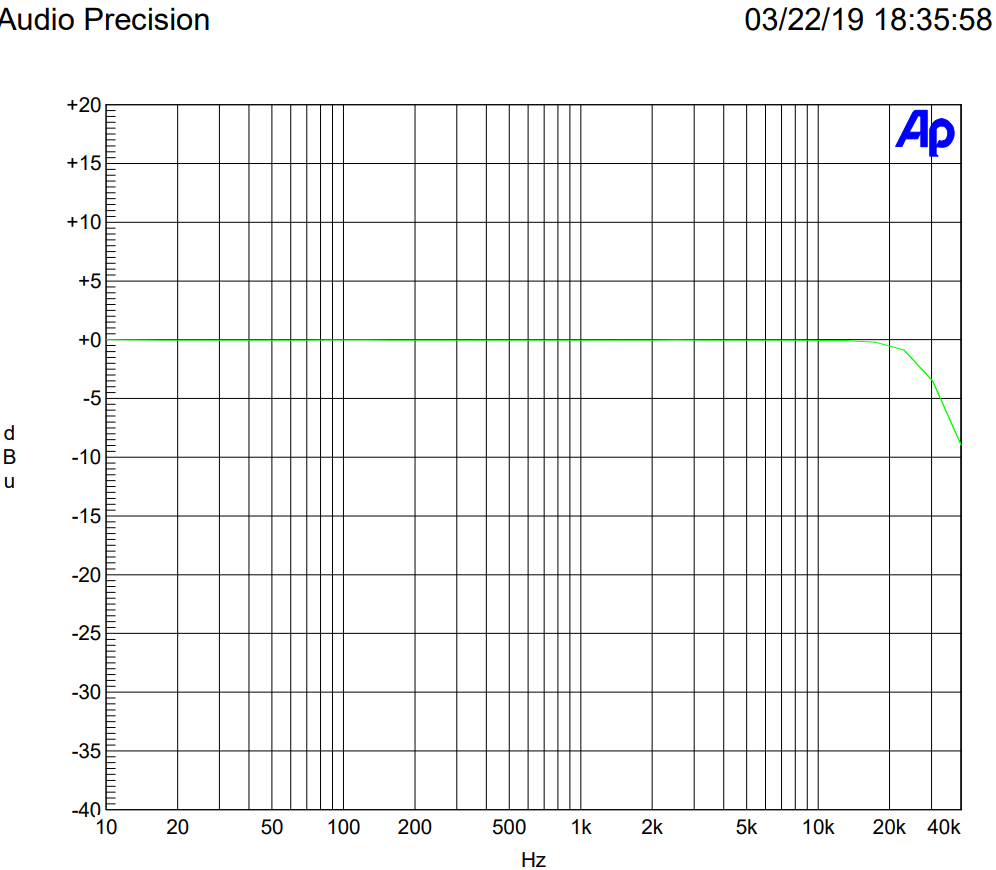
\includegraphics[width = \textwidth]{FinalImages/FR_direct.png}
				\caption{\emph{Direct} routing frequency response measurement output.}
				\label{fig:FR_AP_direct}
			\end{subfigure}
			\begin{subfigure}{0.6\textwidth}
				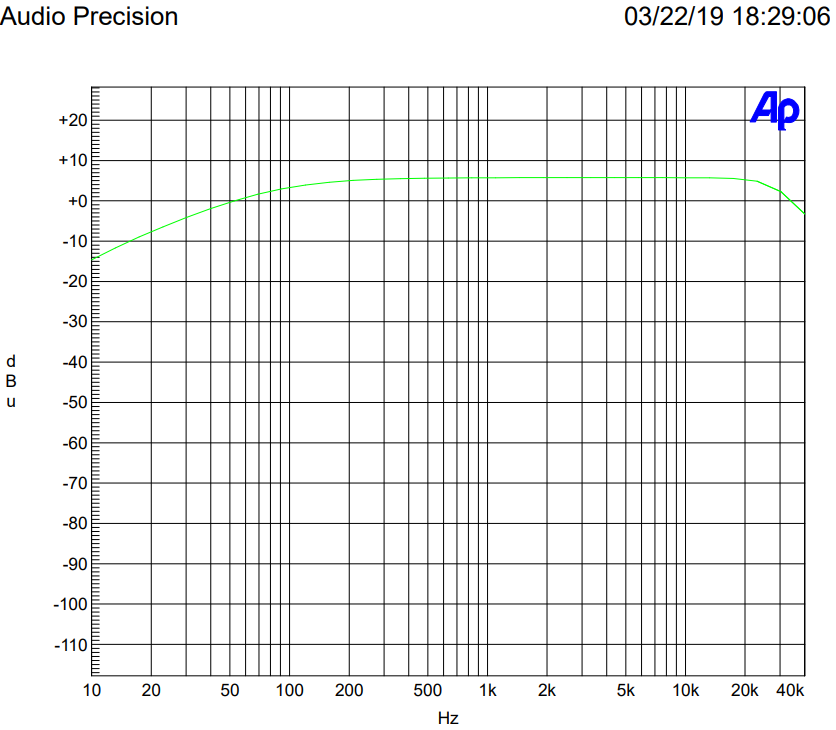
\includegraphics[width = \textwidth]{FinalImages/FR_sum.png}
				\caption{\emph{Summed} routing frequency response measurement output.}
				\label{fig:FR_AP_sum}
			\end{subfigure}
			\caption{Example AP frequency response measurement plots.  The x-axis shows the frequencies of the AP's test sinusoid output amplitude, and the y-axis shows the measured amplitude from the device under test.  Although the high frequency roll off of the \emph{direct} routing appears at first glance to be steeper than that of the \emph{summed} measurement, the scale of the latter plot is longer, so it actuality they have the same slope.  Also note that the flat level of the \emph{summed} test is at $+6dBu$ rather than $0dBu$, which is a result of two $0dBu$ signals being summed.  This means that the latter plot also confirms that the summing amplifier works correctly.}
			\label{fig:FR_AP}
		\end{figure}

		\subsubsection{Analysis}

		To determine if the results of this measurement demonstrate the success or failure of the device to meet the design requirements, the $0.1dBu$ flatness goal was superimposed over the data in the desired frequency range, as seen in .  This was only performed for the \emph{direct} routing configuration, as its accuracy is the most vital.  The rationale for this decision is that when users are using the direct relay-only routing, they are most interested in making subtle comparisons between pedals, so a high performance signal quality specification is paramount.  However, when they use the summing amplifier and splitting features, they are likely more interested in hearing the resulting sound from a combination of pedals, so the signal quality requirements can be slightly relaxed.

		\insertimage{0.8}{PR4Images/FRactive.jpg}{Frequency response of device in active send/receiver mode with signal routing using only relays.  The $0.1dBu$ flatness goal is shown shaded in blue, while the recorded data from the device is plotted as the blue line.  The dashed line at $0dBu$ was the reference signal output by the AP.}{fig:FR_direct}

		As can be seen in Figure \ref{fig:FR_AP_direct}, the device meets this $0.1dBu$ flatness goal.  It makes sense that at no point does the measured signal have a higher amplitude than the reference signal, as the device in this mode is totally passive.  TThe dip in the low frequency is not a big issue, as it occurs around $12Hz$, which is below the audio spectrum, and it still falls within the desired flatness target.

	\subsection{Switching Time}
		\subsubsection{Measurement Description}
		The switching time was measured using the single-shot trigger function of an oscilloscope.  Again the AP was used to output audio signals, in this case sinusoids on both of the channels.  The device output was switched between a direct signal connection to one of the AP outputs and the sum of the two AP outputs.  The trigger level was set higher than the maximum signal level of a single output but below the maximum amplitude of the summed signal.  When the relay switched the output from the single signal to the sum, the oscilloscope triggered and stopped.  The cursors were then used to measure the time difference between when the first signal is lost and begins to float back to ground and when the relay contact stops bouncing and makes solid contact to the second signal.  To capture the relay switching in the opposite direction, one of the AP output signals was inverted so that when the two AP outputs were summed, they canceled, resulting in a lower output.  This was used as the "first" signal, and the trigger level was set to trigger when the relay switched to a single sinusoid.

		\subsubsection{Results}
		Figure 

		\insertimage{0.8}{FinalImages/Switching_oscope.png}{Example oscilloscope trace showing the }



		\subsubsection{Analysis}

		Figure \ref{fig:Switchbar} shows the average switching times with the relays switching in both directions.  Though there does appear to be some asymmetry when switching from one output compared to the other, the measurements show that the switching time is much lower than the $20ms$ goal, and will pose no issue with the signal cutting out.

		\insertimage{0.8}{FinalImages/Switch_bargraph.png}{Comparison of average relay switching time in both directions, plotted with standard deviation.  $N = 20$ for both measurements.  Though there appears to be some difference in the switching times between the two directions, the main takeaway from this plot is that the both of these are far less than the $20ms$ requirement.}{fig:Switchbar}

	\subsection{Switching Transient}

	Transients resulting from signal switching can arise from two main sources. The first is the system itself.  This could result from some microphonic components in the system picking up the mechanical vibrations when the relay blade moves between the contacts. It could also result from the relatively large switching current driving the relay or other digital components coupling into the audio signal. If instead a solid state analog switch had been used, the charge injection resulting from stray capacitances in the MOSFET devices could cause a shift in level, resulting a transient when switched.  The oscilloscope images show that the transient size is never greater than the instantaneous difference between the signals being switched, which demonstrates that the relays themselves do not add any transient.

	The other type of transients are related to the signals themselves that are being switched.  Any instantaneous difference in level will result in a transient of some sort.  The worst possible case would be two signals $180^\circ$ out of phase being switched at the moment they have reached their maximum.  This would result in a transient the size of the signals' amplitude.  Because of time constraints and a desire to avoid adding complexity to minimize signal quality issues, no mitigation circuits were designed to reduce this type of transient.  Measuring this type of switching transient is difficult to glean meaningful data from because of this dependence on the exact signals being switched, so no there was no further exploration of this area during this project.